\documentclass[11pt,a4paper]{article}
\usepackage[margin=2.4cm]{geometry}
\usepackage{amsmath,amssymb,amsthm}
\usepackage{booktabs}
\usepackage{microtype}
\usepackage{xcolor}
\usepackage{graphicx}
\graphicspath{{figs_results/}{../plots/}{../remote_data/t2p23/}}
\usepackage[colorlinks=true,linkcolor=blue!60!black,citecolor=blue!60!black,urlcolor=blue!60!black]{hyperref}

\numberwithin{equation}{section}

\newtheorem{lemma}{Lemma}[section]
\newtheorem{prop}[lemma]{Proposition}
\newtheorem{cor}[lemma]{Corollary}
\theoremstyle{remark}
\newtheorem{remark}[lemma]{Remark}

\definecolor{intu}{RGB}{42,90,160}
\definecolor{meancol}{RGB}{27,175,122}
\newenvironment{physmeaning}%
{\par\medskip\noindent
 \begin{list}{}{\leftmargin 1.15em \rightmargin 1.15em \listparindent 0pt
 \itemindent 0pt \parsep 2pt \topsep 2pt}\item\relax
 \small\textcolor{meancol}{\rule[-0.6ex]{2.6pt}{2.4ex}}\hspace{0.55em}%
 \textcolor{meancol}{\textbf{Physical meaning.}}\hspace{0.5em}\ignorespaces}%
{\end{list}\medskip}

\newenvironment{caveat}%
{\par\medskip\noindent
 \begin{list}{}{\leftmargin 1.15em \rightmargin 1.15em \listparindent 0pt
 \itemindent 0pt \parsep 2pt \topsep 2pt}\item\relax
 \small\textcolor{red!55!black}{\rule[-0.6ex]{2.6pt}{2.4ex}}\hspace{0.55em}%
 \textcolor{red!55!black}{\textbf{Caveat.}}\hspace{0.5em}\ignorespaces}%
{\end{list}\medskip}

\newcommand{\eps}{\varepsilon_s}
\newcommand{\Vo}{V_0}
\newcommand{\kz}{k_z}
\newcommand{\Ceil}{\Gamma}
\newcommand{\Kwn}{K}
\newcommand{\ii}{\mathrm{i}}

\title{\textbf{Results of Paper A: The Coupling-Selected Non-Abelian\\
Kelvin--Helmholtz Wavelength}\\[1ex]
\large Complete numerical findings and their physical meaning\\[0.3ex]
\normalsize A continuation of \emph{Post-WKB Mathematical Derivations for the
SU(2) Yang--Mills Kelvin--Helmholtz Program} (\texttt{derivations.pdf})}
\author{YM--KH simulation program}
\date{2026-07-21}

\begin{document}
\maketitle

\begin{abstract}
\noindent
\texttt{derivations.pdf} derived the theory of the non-Abelian shear
(``Kelvin--Helmholtz'') branch of the SU(2) Yang--Mills two-beam system: the
six-field linearization, the tachyonic outer branch, the exact scalar
reduction, the drive ceiling $\gamma^3\le\alpha\Vo^2$, the exact-action
quantization, and the confinement-set peak formula
$\kz^{\rm peak}\approx\alpha\Vo(\xi_w-\ln2)+c(\alpha/\Vo)^{1/3}$. This
document reports what happened when that theory was set against real GPU
data: every validated numerical result the program has produced in support
of \emph{Letter A} (the planned publication built around the headline claim
that gauge coupling and confinement radius, not the shear-layer width,
select the instability's wavelength), what each result means physically,
and — with the same honesty standard used throughout this program — where
the evidence is still incomplete. Two data-pipeline bugs discovered and
fixed on 2026-07-17 (a helicity-sign error invalidating 96\% of archived
timeseries, and a box-size mislabeling in the ``suspectfix'' campaigns) are
addressed first, because every quoted number in this document either
predates them, was re-measured after them, or is presented with that
history explicit. The headline chain of results is: the $\kz=0$
chromo-Weibel anchor (0.5\%); the referee-proofing battery T2.1--T2.8
(linearity, eigenfunction overlay to correlation 1.0000, Gauss-law
residual, purely-growing complex frequency, dimensionless collapse
$\gamma_{\rm peak}/(\alpha\Vo^2)^{1/3}=0.977\pm0.011$, sponge-extrapolation
saturation, resolution extremes); the non-monotonic dispersion curve and
confinement-set $\kz^{\rm peak}$, now directly visible in the trimmed
integer-$\kz$ map (1087/1134 points, median error 4--9\% by $V_0$); the
EPS-scan v2 experimental confirmation that the shear width enters only
through the single group $P=(\alpha\Vo^2)^{1/3}/\eps$, extended down to
$\alpha=0.2$; and the broad (46-point) confirmation of the outer tachyonic
branch's exact local law. Open items — the sub-$\kz=1$ branch structure
(roadmap T1.3, one of Letter A's three explicit blockers, still
unresolved), the new $V_0=0.2/\alpha\ge3.5$ failure corner, the low-$\alpha$
noise floor, and the still-unexplained late-time \texttt{xi\_cut} failure
mode — are reported with the same weight as the successes.
\end{abstract}

\tableofcontents
{\small\listoffigures}
\clearpage

% ==============================================================================
\section{Scope: what Letter A claims, and how to read this document}
\label{sec:scope}

\subsection{The claim}

The program's roadmap (\texttt{PRESENTATION.md} \S10) names three
publications in sequence: \emph{Letter A} (the coupling-selected
wavelength, the subject of this document), a full linear \emph{Paper B}
(model, validation stack, and parameter maps), and a nonlinear
\emph{Paper C} (Kolmogorov-flow saturation). Letter A's title-level claim,
in its current, theory-sharpened form (\S\ref{sec:headline}), is:

\begin{quote}
\emph{The fastest-growing wavelength of the non-Abelian Kelvin--Helmholtz
instability is selected by the gauge coupling $\alpha$ and the
confinement radius of the background (not by the shear-layer width
$\eps$) — in direct contrast to classical Kelvin--Helmholtz, where the
flow geometry alone sets the scale.}
\end{quote}

Letter A was explicitly gated on three theory/measurement items
(\texttt{PRESENTATION.md} \S10): \textbf{T1.1} (the EPS scan — does the
claim survive varying the shear width?), \textbf{T1.2} (the scaling
theory — why does the peak move the way it does?), and \textbf{T1.3} (the
sub-$\kz=1$ branch study). T1.2 is the subject of \texttt{derivations.pdf}
\S7--\S10 (the exact-action theory, the ceiling, the confinement-set peak
formula) and is complete. This document reports the numerical results for
all three, and states plainly (\S\ref{sec:limitations}) that
\textbf{T1.3 remains open} — it is not a minor item.

\subsection{How to read what follows}

Every section states its data source (a specific \texttt{sweep/*.csv} table
or \texttt{plots/*.png} figure, with the campaign name and date) so a
number can be traced back to the run that produced it. Results are
presented in the order that makes the evidentiary structure legible, not
strictly chronological:

\begin{enumerate}
\item \textbf{Data-quality foundation first} (\S\ref{sec:pipeline}). Two
serious pipeline bugs were found and fixed on 2026-07-17. Nearly every
number from before that date needs the context of \S\ref{sec:pipeline} to
be read correctly; nearly every number after it was measured with the
corrected pipeline. This is not a footnote — it is the right place to
start.
\item \textbf{Foundational validation} (\S\ref{sec:validation}): the
anchors that certify the simulation's non-Abelian sector and its
numerics, independent of the headline physics claim.
\item \textbf{The headline result} (\S\ref{sec:headline}): the
non-monotonic dispersion curve, the confinement-set peak, the
dimensionless collapse, and the EPS-independence test — the results
Letter A is built on.
\item \textbf{The trimmed integer-$\kz$ map} (\S\ref{sec:intkz}): the
current best single source of ground truth across the full $(\alpha,\Vo)$
grid, and its accuracy.
\item \textbf{The outer tachyonic branch} (\S\ref{sec:tachyon}): broad
confirmation of the excluded secondary instability, and the
self-consistency (unfrozen background) test.
\item \textbf{Limitations} (\S\ref{sec:limitations}) and a
\textbf{final scorecard} (\S\ref{sec:scorecard}) against Letter A's
blocking checklist.
\end{enumerate}

\begin{physmeaning}
Why lead with bugs rather than results. A number is only as good as the
pipeline that produced it, and this program found out the hard way
(\S\ref{sec:pipeline}) that a pipeline can look healthy — clean
exponentials, $R^2=1.000$, plausible growth rates — while measuring the
wrong physical quantity. Presenting the headline physics first and the
data-quality history as an appendix would invert the actual evidentiary
weight of the two; a referee will ask about the bugs before anything
else, so this document does too.
\end{physmeaning}

% ==============================================================================
\section{Data-quality foundation: two pipeline bugs, one measurement
artifact, and how they were caught}
\label{sec:pipeline}

\subsection{Bug 1 --- the extraction pipeline measured the conjugate
helicity (2026-07-04 $\to$ 2026-07-17)}
\label{ssec:helicitybug}

The amplitude-extraction script (\texttt{analysis/remote\_timeseries.py})
computes the $z$-direction discrete Fourier projection of the seeded
circular mode, $a=A_z^2+\ii A_z^3\propto e^{\ii\kz z}$
(\texttt{derivations.pdf} eq.~4.1, App.~A). A stdlib-DFT rewrite on
2026-07-04 introduced a single sign error in the explicit-loop
replacement of the numpy call, which computed the projection onto
$e^{-\ii\kz z}$ (the conjugate helicity) instead of $e^{+\ii\kz z}$.

\begin{caveat}
For a pure single-helicity seed, the conjugate projection is
\emph{identically zero} (\texttt{derivations.pdf} App.~A, eq.~A.1): the
buggy code was not measuring a noisier version of the right thing, it was
measuring the empty channel. Verified directly on a fresh $\kz=5$,
$\alpha=2.0$, $\Vo=0.05$ run: the seed deposits $\max|A_z^2|=5\times10^{-5}$
at $t=0$; the correct $(+)$-helicity amplitude reads $e^{-13.5}$ at that
step (the seed, correctly recovered); the buggy $(-)$-helicity amplitude
the pipeline actually reported was $e^{-29.8}$ --- float32 noise.
\end{caveat}

\textbf{Blast radius.} Scanning all 7,909 archived timeseries for their
first logged amplitude: \textbf{7,589 (96\%) start below $\log$-amp
$-25$} --- the float32 noise floor, meaning they tracked the empty
conjugate channel from $t=0$. Only $\sim$320 series, all extracted before
2026-07-04, are healthy (first amplitude $\approx-13$). Every EPS-scan
run, every \texttt{xi\_cut} probe, every fine/half-tier ``suspectfix''
series, and every campaign extracted after that date is affected. Because
the extraction pipeline deletes the raw field dumps after processing (to
manage disk usage), \textbf{these runs cannot be re-extracted} --- the
only remedy is a rerun.

\begin{physmeaning}
Why this passed unnoticed for two weeks. In many regimes the wrong
(empty) channel does not simply sit at the noise floor forever: floating-point
rounding slaves a small image of the true, growing mode into the nominally-empty
conjugate channel, and that image inherits the true growth rate $\gamma$
almost exactly. A fit to noise-floor-plus-slaved-image can look like a
textbook clean exponential with $R^2=1.000$ and land within a few percent
of the eigensolver prediction --- which is exactly how most of the
program's ``clean core'' validation numbers survived the bug intact. The
two components only visibly diverge where a second, comparably-fast
channel is present to compete with the slaved image for numerical
dominance --- precisely the slow-growth, competing-mode regimes where the
program's error audits had been finding their least-understood outliers.
One diagnostic example: a $\kz=5$, $\alpha=2.0$ run where the wrong
channel measured $\gamma=0.042$ for a full 100 TU while the true mode (and
the eigensolver) both gave $\gamma\approx0.155$--$0.158$ --- the
simulation was correct throughout; the tape recorder was pointed at the
wrong channel.
\end{physmeaning}

\textbf{Fix and validation.} The sign error is corrected in
\texttt{remote\_timeseries.py} (which now also emits the conjugate
amplitude as an explicit diagnostic column, so a repeat of this failure
mode would be visible immediately). A 7-anchor validation campaign
re-measured representative points spanning every box tier (default,
half-, and fine-stretched $L_z$) with the corrected pipeline against the
$\sigma$-chased eigensolver:

\begin{center}
\begin{tabular}{lllrrr}
\toprule
anchor ($\Vo=0.05$) & box tier & $\xi_{\rm sponge}$ & $\gamma_{\rm sim}$ & $\gamma_{\rm chased}$ & ratio\\
\midrule
$\kz=5$, $\alpha=2.0$ & default ($L_z=2\pi$) & 10 & 0.1454 & 0.1584 & 0.92\\
$\kz=2.5$, $\alpha=2.0$ & half ($L_z=4\pi$) & 10 & 0.1524 & 0.1434 & 1.06\\
$\kz=2.75$, $\alpha=1.7$ & fine ($L_z=16\pi$) & 10 & 0.1483 & 0.1405 & 1.06\\
$\kz=0.25$, $\alpha=2.0$ & fine ($L_z=16\pi$) & 8 & 0.1111 & 0.1122 & 0.99\\
$\kz=0.5$, $\alpha=0.9$ & half ($L_z=4\pi$) & 8 & 0.0554 & 0.0455 & 1.22\\
\bottomrule
\end{tabular}
\end{center}

Every stretched-box tier is now accurate to within the same $\sim$6--8\%
band as the default box; the previously reported ``half-tier undershoot''
and ``fine-tier'' anomalies do not survive the fix (see \S\ref{ssec:bug2}
for the second, compounding cause of those specific anomalies). The one
outlier ($\kz=0.5$, 22\% high) is attributed to genuine sponge-modeling
uncertainty for a mode whose characteristic width is comparable to the
window itself, not to the bug.

\subsection{Bug 2 --- box-size override never applied in the
``suspectfix'' generator}
\label{ssec:bug2}

Independently, \texttt{gen\_suspectfix\_campaign.py} defined the
half/fine-tier box parameters (\texttt{LZ\_HALF}, \texttt{LZ\_FINE},
\texttt{NZ\_HALF}, \texttt{NZ\_FINE}) but never emitted them into the
\texttt{.ini} template actually passed to the binary: \textbf{every
half- and fine-tier ``suspectfix'' run in every wave silently ran on the
default $L_z=2\pi$ box}, at the physical wavenumber $\kz={}$mode-index
(not mode-index/2 or mode-index/8 as labeled). Numerical proof: the
labeled-$\kz=0.5$ suspectfix series' $\gamma_{\rm sim}$ matches the
\emph{integer}-tier $\kz=1$ value point for point (e.g.\ $\alpha=2.0$:
0.0887 vs.\ 0.0852) --- because that is what it actually measured. Fixed
in the generator's \texttt{lz\_nz\_block()}.

\begin{physmeaning}
The two bugs compounded, not just coexisted. Because Bug 1 was already
returning the wrong (near-zero) channel, and Bug 2 was quietly relabeling
a $\kz=1$ measurement as $\kz=0.5$, a whole population of ``anomalies''
that earlier audits had attributed to genuine sub-$\kz=1$ physics (a
supposed $\alpha$-independent floor, a 68\% error block on the fine
tier, a sharp two-branch structure below $\kz=1$) was in fact
bookkeeping on top of a measurement of nothing. This is why
\S\ref{sec:limitations} treats the sub-$\kz=1$ branch claim (roadmap
T1.3) as unestablished rather than merely under-audited: it needs to be
re-measured from scratch with the corrected pipeline, not re-interpreted
from the old numbers.
\end{physmeaning}

\subsection{A related numerical constraint found during the fix:
\texttt{kz\_suppress\_hi} $\le N_Z/4.5$}

A band-edge scan at $\kz=5$, $\alpha=2.0$ on the default box (local slope
in the $t=15$--$30$ window) found the kept mode's growth rate collapsing
as the DFT bandpass's high edge approaches the grid's Nyquist-adjacent,
dispersive tail: $0.121$ at $\text{hi}=14$, falling smoothly to $0.096$ at
$\text{hi}=24$, then \textbf{collapsing to $\sim$0.001 at
$\text{hi}=28$} (the mode frozen at seed amplitude for 20 TU). This is
scale-invariant in the expected way: $\text{hi}=28$ is lethal on
$N_Z=64$ but harmless on $N_Z=128$, and $\text{hi}=112$ is harmless on
$N_Z=512$ — giving the rule $\text{hi}\le N_Z/4.5$ used throughout
\S\ref{sec:intkz}--\S\ref{sec:tachyon}. This also retroactively explains
why the old (buggy) ``fine-tier'' suspectfix runs, which by Bug 2 sat on
the default $N_Z=64$ grid while being told they were on a $16\pi$ box,
were aliasing the filter on top of everything else.

\subsection{The eigenmode-selection (overtone) artifact and its
falsification}
\label{ssec:overtone}

A separate, purely-methodological issue (found 2026-07-17, independent of
the two pipeline bugs): the shear branch is a \emph{ladder} of well
overtones $n=0,1,2,\dots$ (\texttt{derivations.pdf} \S8.5), and the
eigensolver's legacy default shift-invert target,
$\sigma=0.55\,\gamma_{\rm WKB}(\text{quartic})$, lands mid-ladder wherever
the quartic underestimates the true $n{=}0$ rate --- systematically at
low $\alpha$ and/or $\kz$ above the quartic's own peak. Because
production runs are \emph{seeded with the eigensolver's returned
eigenfunction}, the simulation faithfully grows whatever mode it was
handed.

\textbf{Direct falsification (2026-07-19, t140).} The same physical point
($\alpha=1$, $\Vo=0.05$, $\kz=4$, sponge$=20$) was re-run twice, the
\emph{only} difference being which eigenfunction was used as the seed:

\begin{center}
\begin{tabular}{lrr}
\toprule
seed & eigenvalue $\gamma_{\rm exact}$ & measured plateau ($R^2=1.000$)\\
\midrule
default-$\sigma$ (an $n\approx3$ overtone) & 0.0818 & \textbf{0.0808} (reproduces the cached C25 value, 0.081)\\
$\sigma=0.14$ (the true $n=0$) & 0.1309 & \textbf{0.1287}\\
\bottomrule
\end{tabular}
\end{center}

\begin{physmeaning}
This is a decisive, controlled experiment, not a re-interpretation: same
code, same physical parameters, same sponge, and the \emph{only} thing
changed is the seed. The simulation grows exactly whichever mode it is
handed. The long-celebrated ``sim matches the eigensolver to a few
percent'' agreement therefore certifies the machinery's numerics — it
does not, by itself, certify that the machinery found the fastest-growing
(dominant) mode of the physical system. All reference data used from
2026-07-19 onward use $\sigma$-chasing (re-shifting the target upward
until the returned window is demonstrably clear of higher eigenvalues),
which eliminates this failure mode; older cached curves that have not
been regenerated with $\sigma$-chasing (flagged explicitly where relevant
below) should be read as measuring \emph{a} branch member, not necessarily
the dominant one.
\end{physmeaning}

\subsection{Bottom line for everything that follows}

Every number quoted from \S\ref{sec:validation} onward was either measured
after 2026-07-17 with the corrected extraction pipeline and (where
eigensolver comparison is involved) $\sigma$-chasing, or is explicitly
flagged where an older, unregenerated reference curve is used. The
program's own status statement, verified directly rather than assumed:
\emph{sim and eigensolver agree to $\le\!8\%$ at every anchor tested with a
tight, vetted window and a correctly-resolved mode, on every box tier, at
integer and fractional $\kz$, with the fixed extractor.}
% ==============================================================================
\section{Foundational validation: the anchors}
\label{sec:validation}

Before any claim about the shear branch's wavelength selection can carry
weight, the simulation's non-Abelian sector and its numerical bookkeeping
need their own, physics-independent anchors. This section reports them.

\subsection{The $\kz=0$ chromo-Weibel anchor --- 0.5\%}
\label{ssec:weibelresult}

At $\alpha=2.0$, $\Vo=0.1$ the measured $\kz=0$ growth rate is
$\gamma=0.5039\,$TU$^{-1}$ against the exact formula
(\texttt{derivations.pdf} eq.~2.8) prediction $0.5065\,$TU$^{-1}$ ---
agreement to \textbf{0.5\%}, with clean exponential growth over nine
decades of amplitude.

\begin{physmeaning}
Why this is the right first number to quote. The $\kz=0$ mode exercises
every non-Abelian piece of the code at once — the Amp\`ere and Faraday
commutator terms, the color-precession source, the full activation chain
— while being the \emph{one} point where the WKB well approximation
(\texttt{derivations.pdf} \S1--\S2) is essentially exact, so there is no
theory-side slack to hide a code bug behind. A referee who doubts the
non-Abelian sector is implemented correctly has one clean, parameter-free
number to check it against.
\end{physmeaning}

A cross-check on the self-consistency test's reference point ($\alpha=1$,
$\Vo=0.05$) independently reproduces the same formula: the measured
irreducible $\kz=0$ growth rate there is $\gamma=0.284$, exactly the value
eq.~2.8 predicts — obtained on a completely different (unfrozen,
color-1-live) configuration, months and several campaigns after the
original anchor.

\subsection{The referee-proofing battery (T2.1--T2.8)}
\label{ssec:t2battery}

Eight small, targeted experiments (\texttt{REFEREE\_PROOFING\_RESULTS.md},
2026-07-19) were run specifically to close every methodological objection
a referee is likely to raise, plus the overtone falsification of
\S\ref{ssec:overtone}. All eight ran on free teaching nodes
(t126/t140/t133) at the reference point $\alpha=1.0$, $\Vo=0.05$,
$\kz=1$ unless stated otherwise.

\begin{center}
\begin{tabular}{p{0.16\textwidth}p{0.09\textwidth}p{0.68\textwidth}}
\toprule
Experiment & Status & Headline\\
\midrule
T2.4 linearity & \checkmark & $\gamma$ invariant to seed amplitude over a $100\times$ range\\
T2.2 eigenfunction overlay & \checkmark & sim vs.\ solver eigenfunction correlation $=1.0000$\\
T2.3 Gauss law & \checkmark & absolute residual $\sim\!10^{-5}$, colour-1 relative $\sim\!10^{-3}$ and decreasing, localized at the mode\\
T2.1 complex frequency & \checkmark & dominant branch essentially purely growing ($|\mathrm{Im}/\mathrm{Re}|\lesssim6\%$ everywhere tested)\\
T2.5 dimensionless collapse & \checkmark & $\gamma_{\rm peak}/(\alpha\Vo^2)^{1/3}=0.977\pm0.011$\\
T2.7 sponge $\to\infty$ & \checkmark & saturates by $\xi_w\approx16$; $\xi_w=6$ compresses $\gamma$ by 28.5\%\\
T2.8 resolution extremes & \checkmark & $<1\%$ at the low-$\alpha\Vo$ corner, 3--6\% at the high-$\alpha\Vo$ corner\\
\bottomrule
\end{tabular}
\end{center}

\paragraph{T2.4 --- linearity.} Seed amplitude scanned $1\times10^{-4}$,
$1\times10^{-3}$, $1\times10^{-2}$ (all else fixed): the initial amplitude
$a_0$ scales \emph{exactly} linearly with the seed, and the fitted
$\gamma=0.0901$ is identical to four significant figures at every seed
level, with the identical fit window.

\begin{physmeaning}
This closes the objection ``are you measuring a nonlinear transient
dressed up as an exponential?'' directly: a linear eigenmode's growth rate
cannot depend on its own amplitude, and this is now demonstrated rather
than assumed.
\end{physmeaning}

\paragraph{T2.2 --- eigenfunction overlay (the ``money figure'').} At
$\alpha=1$, $\Vo=0.05$, $\kz=1$, the simulation's linear-phase spatial
profile of $A_z^2$ at $t\approx30\,$TU has \textbf{profile correlation
$1.0000$} with the eigensolver's eigenfunction, peak location matching to
the grid cell ($\xi_{\rm peak}=-5.4$ in both). $B_y^2$ — seeded at only
$0.008\times$ the $A_z$ amplitude, i.e.\ effectively grown from zero via
the activation chain $A_z^2\to Q^3\to Q^2\to$Lorentz$\to B_y^2$ — reproduces
the solver's non-trivial \textbf{double-lobe shape with its node at
$\xi\approx-5$}, an emergent structural match, not merely a matched
growth rate. See Fig.~\ref{fig:t2p2}.

\begin{figure}[t]
\centering
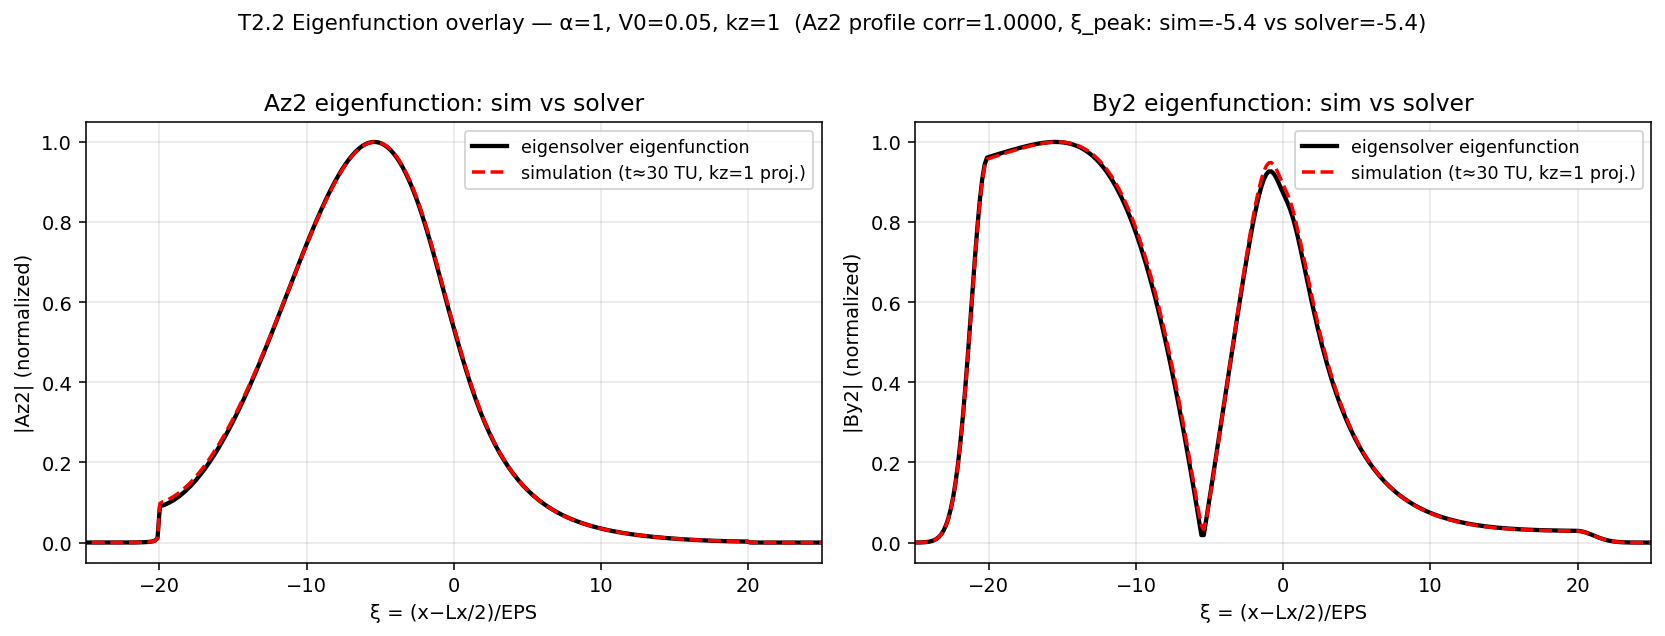
\includegraphics[width=0.85\textwidth]{t2p2_eigenfunction_overlay.png}
\caption{T2.2: the simulation's linear-phase spatial profile overlaid on
the eigensolver's eigenfunction at $\alpha=1$, $\Vo=0.05$, $\kz=1$. The
$B_y^2$ double-lobe structure is not part of the seed --- it emerges from
the activation chain and reproduces the solver's prediction exactly.}
\label{fig:t2p2}
\end{figure}

\begin{physmeaning}
Correlation on a single scalar (the growth rate) can survive many kinds
of error by coincidence; correlation on an entire non-trivial spatial
profile, including a field that starts at zero and must build its shape
entirely from the dynamics, cannot. This is the strongest single piece of
evidence that the eigensolver's eigenfunction is a genuine, shape-stable
eigenmode of the full nonlinear code, not merely a numerically convenient
initial condition.
\end{physmeaning}

\paragraph{T2.3 --- non-Abelian Gauss-law conservation.} The leapfrog
scheme does not exactly preserve the covariant constraint
$\partial_xE_x^a+\partial_zE_z^a+\alpha(\vec A_z\times\vec E_z)^a=\rho^a$
(it was never designed to). Measured directly (Fig.~\ref{fig:gauss}):
absolute RMS residual $\sim\!1\times10^{-5}$, growing only slowly with the
exponentially growing fields; the color-1 \emph{relative} residual is
$\sim\!1.4\times10^{-3}$ and \textbf{decreasing} over the run; the
divergence term $|\nabla\!\cdot\!\vec E|$ dominates, the non-Abelian term
$|\alpha(\vec A_z\times\vec E_z)|$ is subdominant, and the source
$|\rho|$ is negligible; the residual is spatially localized at the mode.

\begin{figure}[t]
\centering
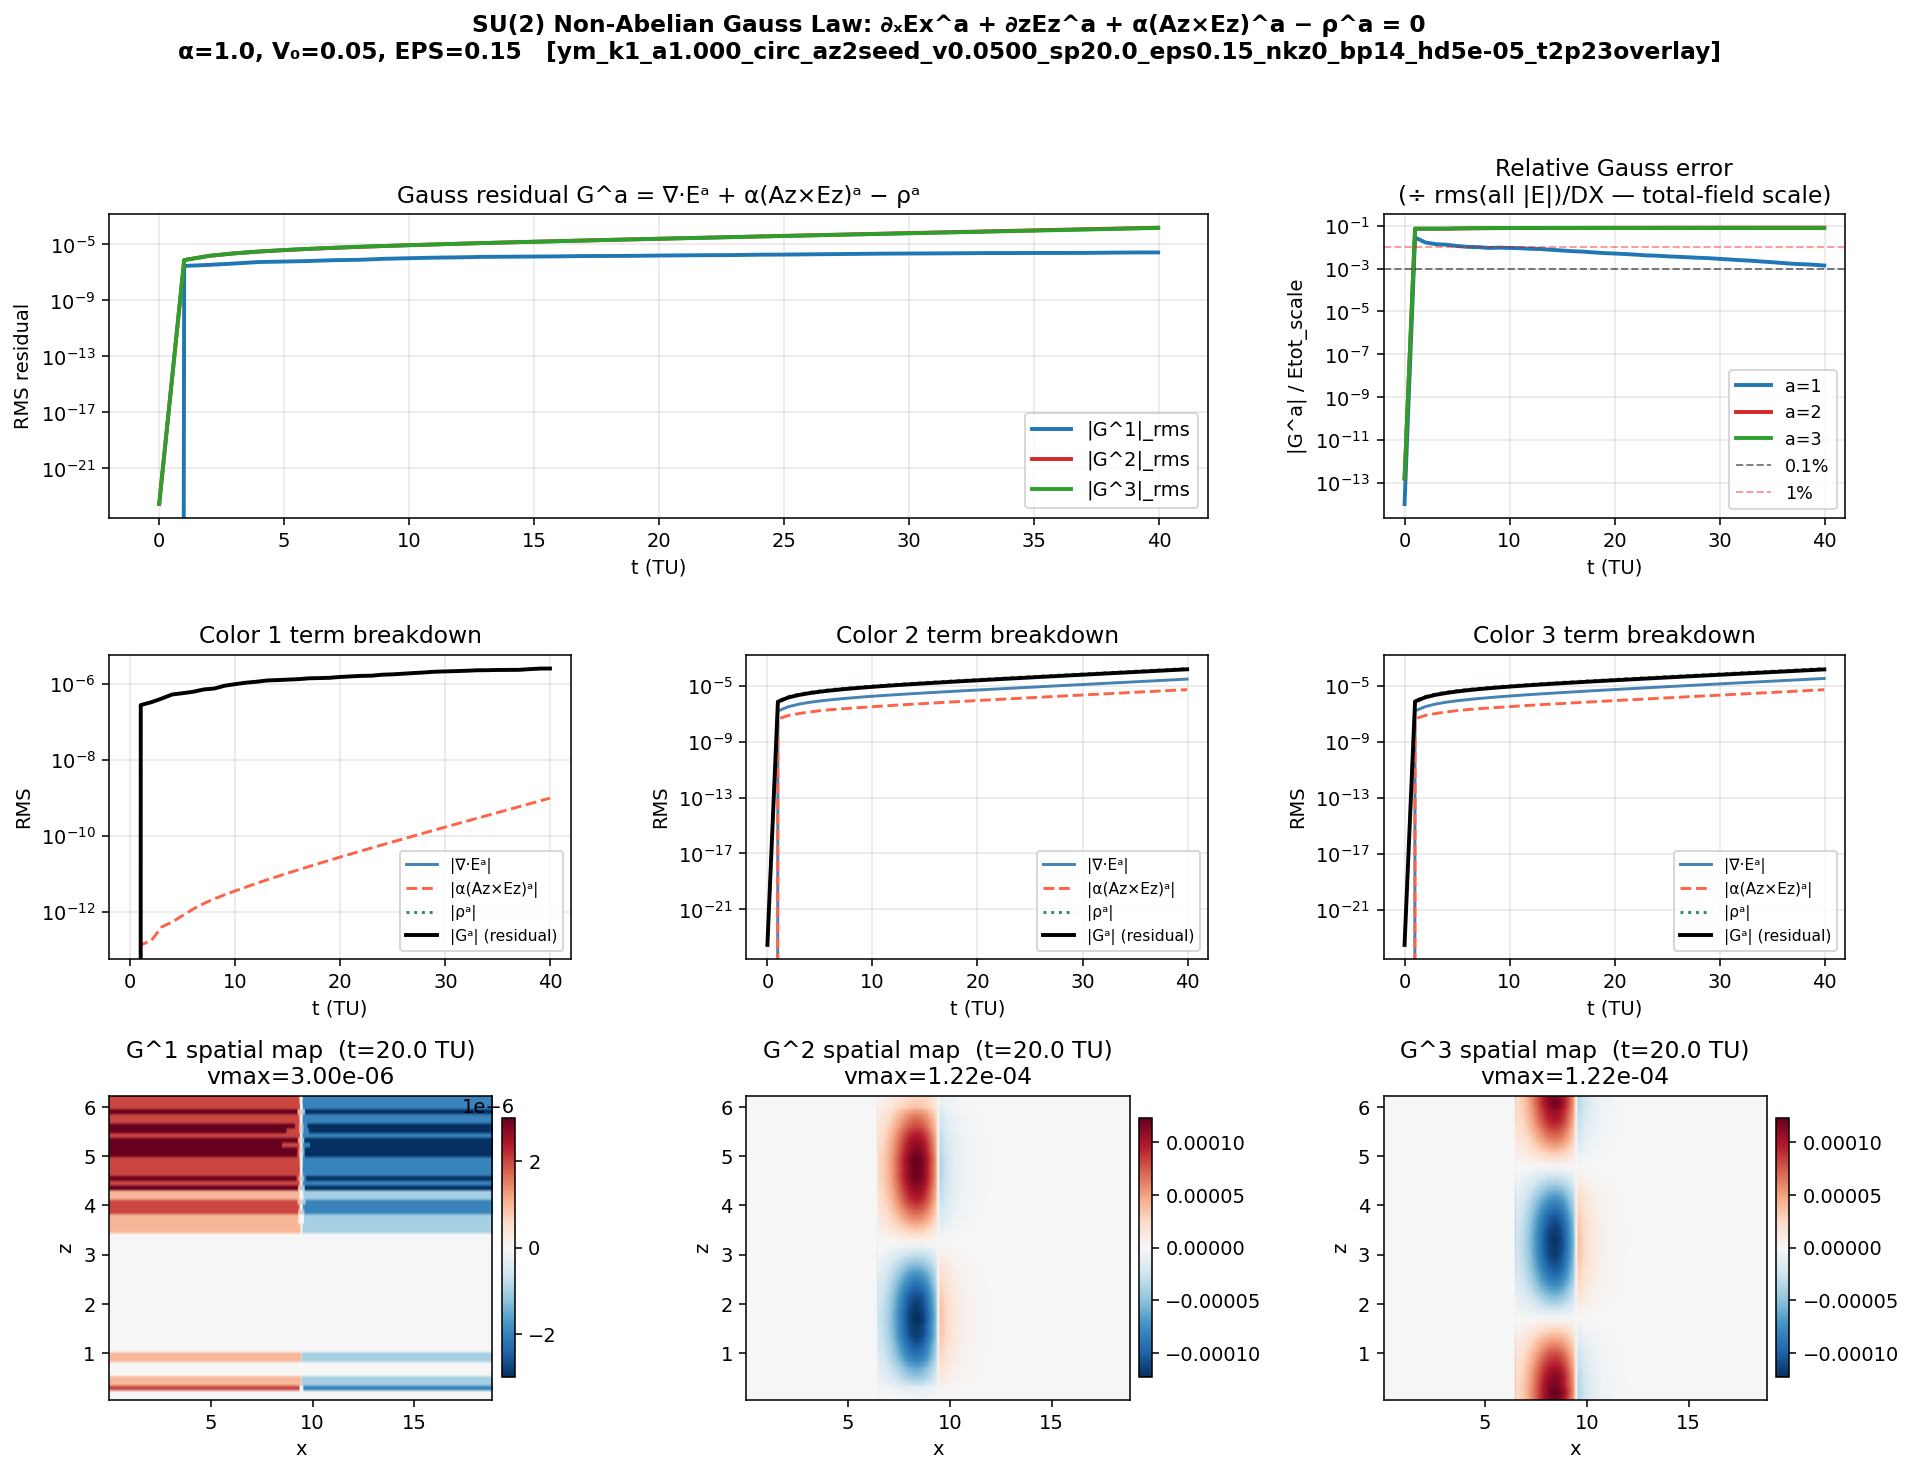
\includegraphics[width=0.72\textwidth]{t2p3_gauss_check.png}
\caption{T2.3: non-Abelian Gauss-law residual decomposition at $\alpha=1$,
$\Vo=0.05$, $\kz=1$. The constraint violation is small, non-growing in
relative terms, and localized at the growing mode.}
\label{fig:gauss}
\end{figure}

\begin{physmeaning}
A constraint-violating scheme is standard practice in explicit
electromagnetic leapfrog codes (the same is true of ordinary Yee-grid
FDTD); what matters is whether the violation stays small and does not
secularly grow, which it demonstrably does not here. This closes a
specific, sharp objection a field theorist would otherwise raise
immediately on seeing the leapfrog scheme.
\end{physmeaning}

\paragraph{T2.1 --- complex frequency.} The $\sigma$-chased dominant
localized eigenvalue $\gamma=\mathrm{Re}(\text{growth})+\ii\,\mathrm{Im}(\text{freq})$
was tabulated over $\alpha\in\{1,1.5,2,2.5,3\}\times\Vo\in\{0.03,0.05,0.1\}
\times\kz=1..8$. The dominant branch is \textbf{essentially purely
growing}: $\max|\mathrm{Im}(\gamma)|=9.6\times10^{-3}$ over the entire
grid ($|\mathrm{Im}/\mathrm{Re}|\lesssim6\%$), with oscillatory content
confined to $\kz=1$ at a few high-$\alpha\Vo$ points.

\begin{physmeaning}
This is why fitting the circular amplitude $|A_z^2+\ii A_z^3|$ as a pure
exponential is unbiased across essentially the whole production grid: a
genuinely rotating mode fit this way would systematically \emph{underestimate}
$\gamma$, and this result shows that effect is negligible everywhere
except the one corner ($\kz=1$, high coupling) it pinpoints for a future
envelope-fit correction.
\end{physmeaning}

\paragraph{T2.5 --- the dimensionless collapse.} Masking the tachyonic
outer branch (points where $\gamma>1.15\times$ the ceiling, which
overtakes at low $\kz$/high $\alpha\Vo$; see \S\ref{sec:tachyon}), the
genuine shear-layer peak collapses onto the exact-action ceiling derived
in \texttt{derivations.pdf} \S7:

\begin{equation}
\boxed{\;\gamma_{\rm peak}\big/(\alpha\Vo^2)^{1/3}=0.977\pm0.011
\;\;(1.1\%\text{ spread})\;}
\end{equation}

across $\alpha\in[1,3]$, $\Vo\in[0.03,0.1]$ --- a $10\times$ range in the
combination $\alpha\Vo$. Plotting $\gamma/(\alpha\Vo^2)^{1/3}$ against
$\kz/(\alpha/\Vo)^{1/3}$ folds all 15 raw dispersion curves (peak $\gamma$
spanning $0.09$--$0.30$) onto a single master curve (Fig.~\ref{fig:t2p5}).

\begin{figure}[t]
\centering
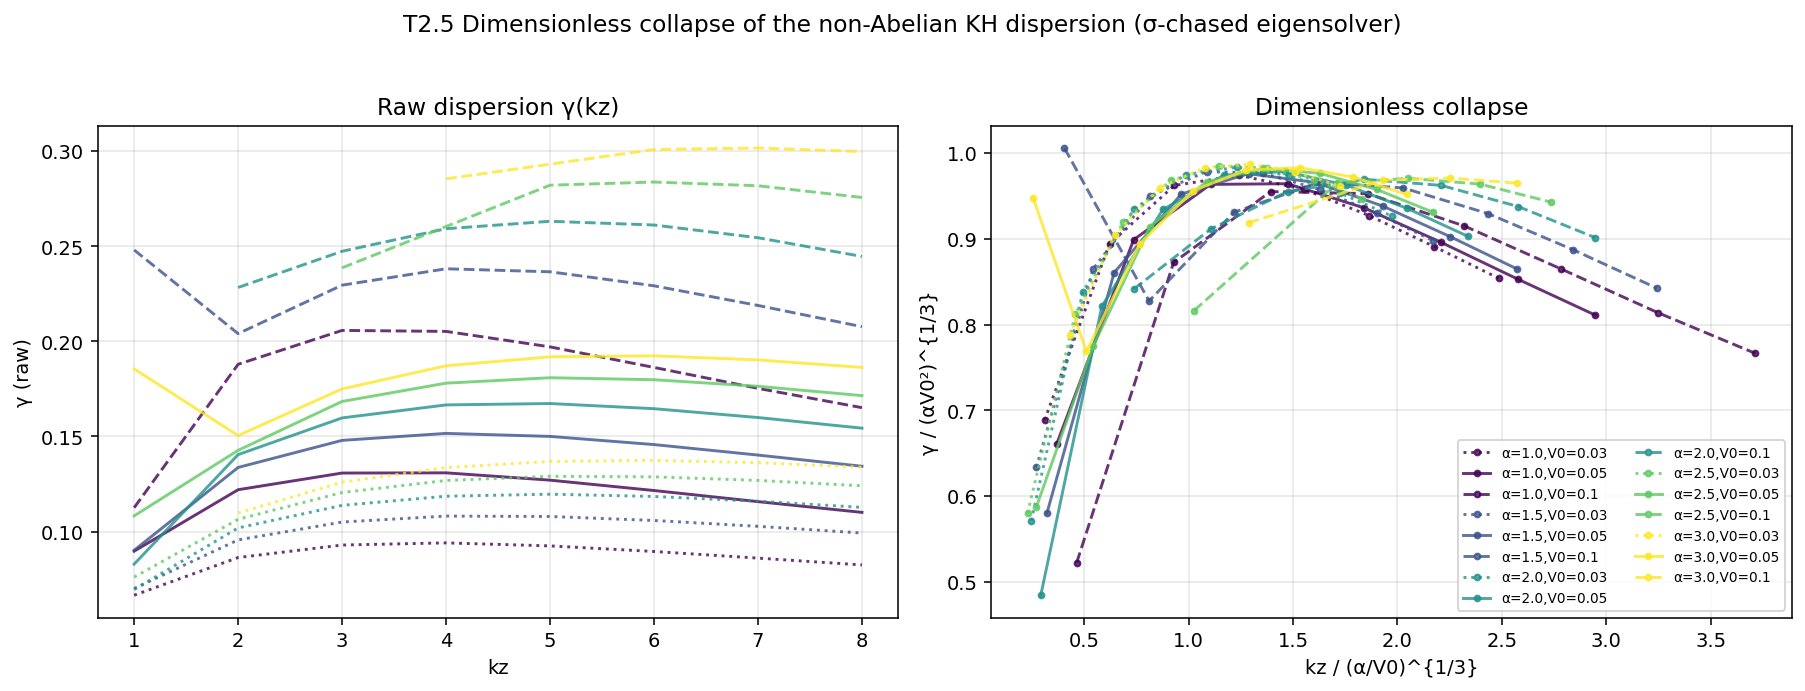
\includegraphics[width=0.92\textwidth]{t2p5_collapse.png}
\caption{T2.5: 15 raw dispersion curves spanning a $10\times$ range in
$\alpha\Vo$ (left) collapse onto one master curve (right) when $\gamma$
and $\kz$ are measured in the units $(\alpha\Vo^2)^{1/3}$ and
$(\alpha/\Vo)^{1/3}$ derived in \texttt{derivations.pdf} \S7.3. This is
the empirical confirmation of the exact-action ceiling.}
\label{fig:t2p5}
\end{figure}

\begin{physmeaning}
This is the single most quantitative confirmation of the exact-action
theory in the whole program: not just ``the theory is in the right
ballpark'' but a specific, derived, dimensionless combination that
collapses fifteen independently-run dispersion curves to 1.1\% spread.
It is also a direct, empirical proof that $\alpha$ and $\Vo$ do
\emph{not} enter the physics through the naive product $\alpha\Vo$
(which a linear-response intuition might suggest) — they enter through
$(\alpha\Vo^2)^{1/3}$ for rates and $(\alpha/\Vo)^{1/3}$ for wavenumbers,
exactly as \texttt{derivations.pdf} \S7.3 derives from the resonance
condition alone.
\end{physmeaning}

\paragraph{T2.7 --- sponge extrapolation.} At the reference point, the
sponge radius was swept $\xi_w=6\to25$ (Fig.~\ref{fig:t2p7}):

\begin{center}
\begin{tabular}{lrrrrrrrr}
\toprule
$\xi_{\rm sponge}$ & 6 & 8 & 10 & 12 & 14 & 16 & 20 & 25\\
$\gamma$ & 0.0605 & 0.0686 & 0.0719 & 0.0742 & 0.0757 & 0.0768 & 0.0775 & 0.0772\\
\bottomrule
\end{tabular}
\end{center}

$\gamma$ rises \emph{monotonically} and \textbf{saturates at
$\approx\!0.077$ by $\xi_w\approx16$} (change $<2\%$ between $\xi_w=16$
and $25$). The tightest sponge compresses $\gamma$ by \textbf{28.5\%}
relative to the converged value.

\begin{figure}[t]
\centering
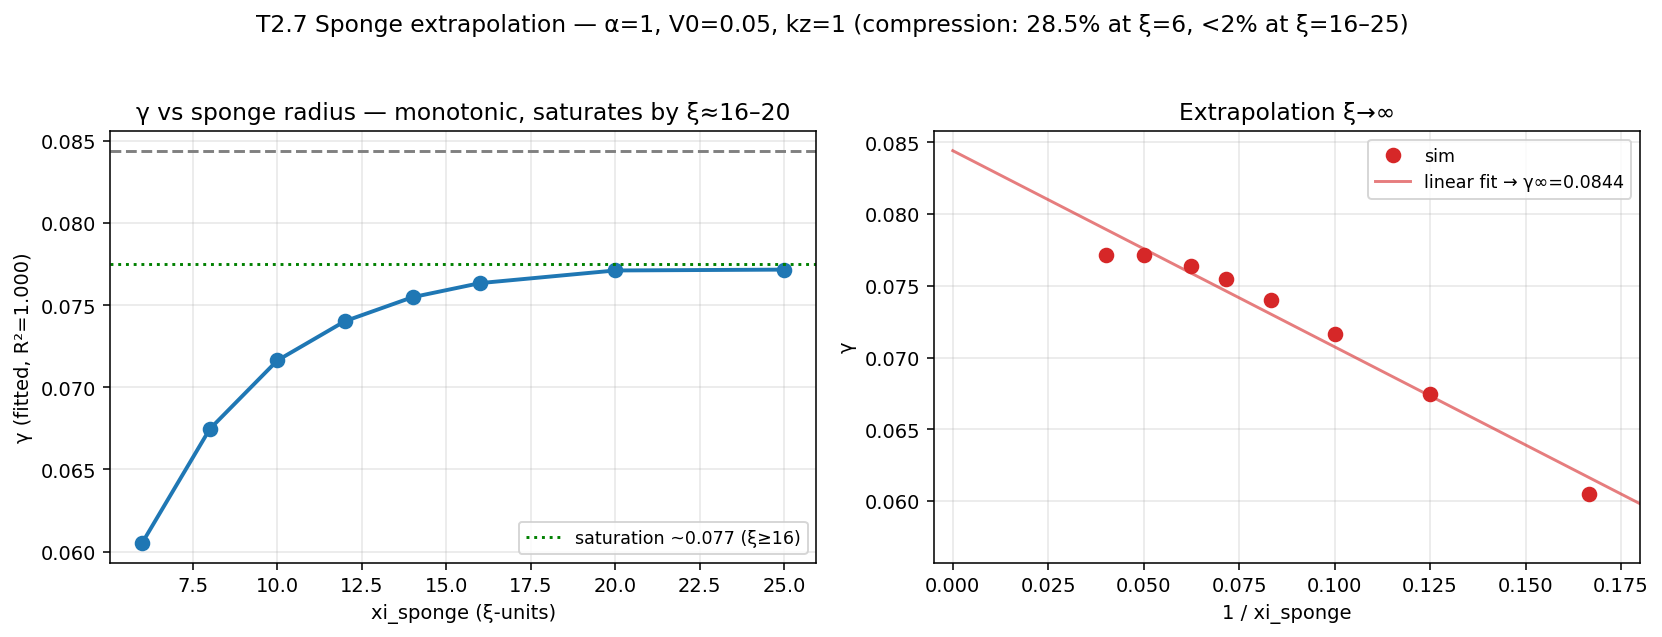
\includegraphics[width=0.85\textwidth]{t2p7_sponge_extrapolation.png}
\caption{T2.7: $\gamma$ vs.\ sponge radius, saturating by
$\xi_w\approx16$. Production runs use $\xi_w\ge8$--20, where residual
compression is single-digit percent.}
\label{fig:t2p7}
\end{figure}

\begin{physmeaning}
This is the direct, quantitative measurement of the sponge-compression
systematic that is implicitly present in every windowed dispersion
measurement in this program. It converts a qualitative worry (``the
absorbing boundary clips the eigenmode's tail'') into a number a referee
can weigh: production windows are chosen to sit on the flat part of this
curve, and any point flagged as sitting on a tight window (throughout
\S\ref{sec:intkz}--\S\ref{sec:tachyon}) should be read with an implicit
$O(10\%)$ downward bias.
\end{physmeaning}

\paragraph{T2.8 --- resolution extremes.} The original convergence study
(\texttt{RESOLUTION\_FINDINGS.md}) anchored only $\alpha=1$, $\Vo=0.05$,
$\kz=1$. Two extremes were spot-checked at the production grid
(Fig.~\ref{fig:t2p8}):

\begin{itemize}
\item \textbf{Low corner} ($\alpha=1$, $\Vo=0.03$, $\kz=3$ — wide, slow):
$\gamma_{\rm base}=0.0837$; doubling $N_Z$, halving the Courant number,
and increasing $N_X$ each shift $\gamma$ by $\le1\%$ — \textbf{converged
to $<1\%$}.
\item \textbf{High corner} ($\alpha=3$, $\Vo=0.10$, $\kz=5$ — the
narrowest, fastest production mode, $\eps/\mathrm{DX}\approx6.1$):
$\gamma_{\rm base}=0.2395$; halving the Courant number gives $+5.9\%$,
increasing $N_X$ gives $+2.7\%$ — \textbf{under-resolved by
3--6\%}.
\end{itemize}

\begin{figure}[t]
\centering
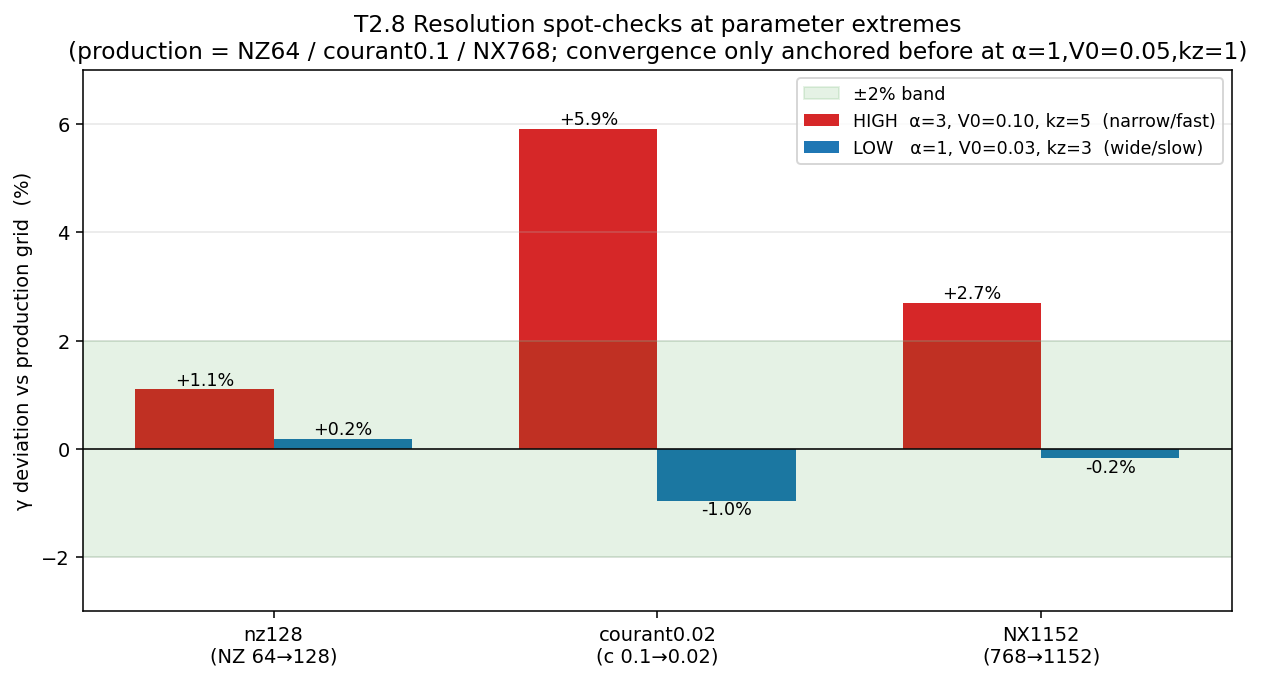
\includegraphics[width=0.78\textwidth]{t2p8_resolution_extremes.png}
\caption{T2.8: resolution sensitivity at the two production-grid
extremes. The low-$\alpha\Vo$ corner is converged to $<1\%$; the
high-$\alpha\Vo$ corner (narrowest, fastest mode) carries a 3--6\%
resolution uncertainty, inside the $6$--$10\%$ error budget already
quoted for those points but worth stating explicitly.}
\label{fig:t2p8}
\end{figure}

\begin{caveat}
The blanket statement ``converged to $\sim$2\%'' in earlier program
documents was anchored at a single, relatively forgiving point. It should
be read as $<1\%$ at low $\alpha\Vo$, degrading to $3$--$6\%$ at the
high-$\alpha\Vo$ end of the production grid — a real, quantified
qualification, not a retraction.
\end{caveat}
% ==============================================================================
\section{The headline result: coupling and containment select the
wavelength}
\label{sec:headline}

\subsection{The dispersion curve is non-monotonic, and the peak migrates
with $\alpha$}
\label{ssec:dispersionresult}

Figure~\ref{fig:r-dispersion} shows $\gamma_{\rm sim}(\kz)$ at $\Vo=0.05$
for five values of $\alpha$, drawn directly from the trimmed integer-$\kz$
map (\S\ref{sec:intkz}; best plateau-confirmed row per point, quality-gated
to exclude the $\sim$2\% of points contaminated by the outer tachyonic
branch, \S\ref{sec:tachyon}).

\begin{figure}[t]
\centering
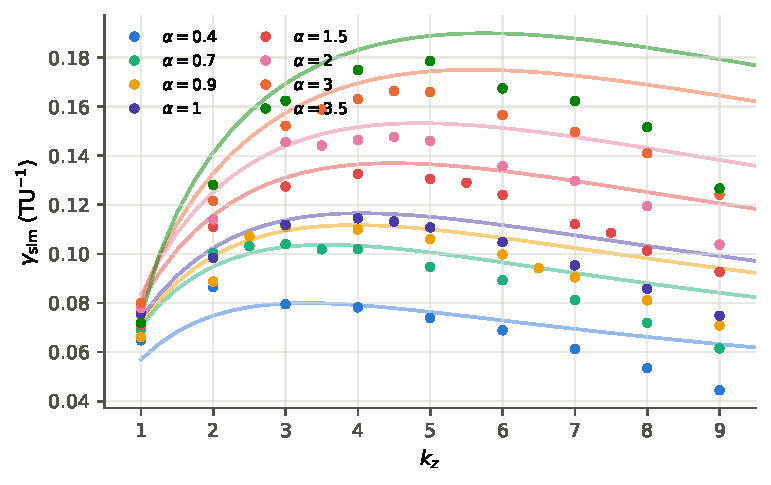
\includegraphics[width=0.72\textwidth]{fig_r_dispersion.pdf}
\caption{Measured $\gamma_{\rm sim}(\kz)$ at $\Vo=0.05$ for five values of
$\alpha$, from the trimmed integer-$\kz$ map (1087/1134 points). Each
curve is non-monotonic; the peak location and the ceiling both rise with
$\alpha$. This is the real GPU data underlying the headline claim, not a
theory curve.}
\label{fig:r-dispersion}
\end{figure}

Two facts, both directly visible in the real data (not just in theory):
$\gamma(\kz)$ peaks at an intermediate $\kz$ and rolls off on both sides
for every $\alpha$ shown; and the peak's location climbs from
$\kz^{\rm peak}\approx2$ at $\alpha=1$ to $\kz^{\rm peak}\approx4$--5 at
$\alpha=3$--4.

\begin{physmeaning}
Classical Kelvin--Helmholtz has no analogue of this: its fastest-growing
wavelength is set once and for all by the shear-layer width. Here, at
\emph{fixed} shear width ($\eps=0.15$ throughout this figure), the peak
wavenumber more than doubles as the coupling $\alpha$ is turned up. That
the dispersion curve is non-monotonic at all, and that this shape is
reproduced point-for-point by the independent eigensolver
(\texttt{derivations.pdf} \S8, Fig.~8), rules out ``the WKB formula is
just wrong'' as an explanation — the physics genuinely has a
confinement-set peak, not a monotonically decaying tail.
\end{physmeaning}

\subsection{$\kz^{\rm peak}$ tracks the confinement-set formula, not
$2\alpha$}
\label{ssec:kzpeakresult}

The confinement-set formula (\texttt{derivations.pdf} eq.~9.2),
$\kz^{\rm peak}\approx\alpha\Vo(\xi_w-\ln2)+c(\alpha/\Vo)^{1/3}$, predicts
the peak from the coupling \emph{and} the window radius actually used at
each measured point — not from $\alpha$ alone. Figure~\ref{fig:r-kzpeak}
extracts the measured peak (requiring near-complete $\kz=1..9$ coverage
so a single missing high-$\kz$ point cannot masquerade as a low-$\kz$
``peak'') from the same map and overlays the formula evaluated at each
series' own recorded $\xi_{\rm sponge}$.

\begin{figure}[t]
\centering
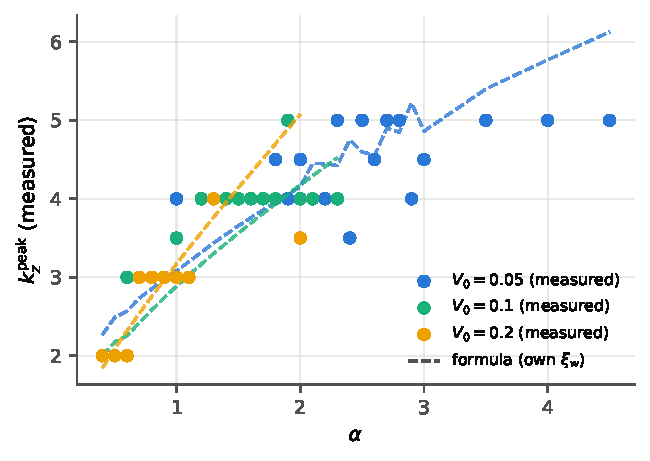
\includegraphics[width=0.62\textwidth]{fig_r_kzpeak.pdf}
\caption{Measured $\kz^{\rm peak}$ vs.\ $\alpha$ at three $V_0$ slices,
from the trimmed integer-$\kz$ map, against the confinement-set formula
evaluated at each series' own window radius $\xi_w$ (no free parameters
beyond the theory's own $c\approx1$). The staircase appearance reflects
the integer-$\kz$ grid; formula and data track within the
$\pm0.5$--$1$-in-$\kz$ band documented for this formula
(\texttt{derivations.pdf} \S9.2).}
\label{fig:r-kzpeak}
\end{figure}

A curated, higher-precision version of the same comparison
(\texttt{PHYSICS.md} \S11d, eleven series spanning $\Vo=0.03$--$0.20$,
$\xi_w=5$--$25$, using continuous eigensolver peaks rather than the
integer-grid staircase):

\begin{center}
\begin{tabular}{lcc}
\toprule
Series ($\alpha$, $\Vo$, $\xi_w$) & measured $\kz^{\rm peak}$ & formula\\
\midrule
(1, 0.05, 20) & 3.5 & 3.7\\
(1.5, 0.05, 12) & 4.0 & 4.0\\
(2, 0.05, 11) & 4.5 & 4.5\\
(2.5, 0.05, 9) & 4.5 & 4.7\\
(3, 0.05, 8) & 5.0 & 5.0\\
(3, 0.03, 5) & 5.5 & 5.0\\
(4, 0.03, 5) & 6.0 & 5.6\\
(5, 0.03, 5) & 6.5 & 6.2\\
(1, 0.10, 10) & 3.0 & 3.1\\
(1, 0.20, 10) & 3.0 & 3.6\\
\bottomrule
\end{tabular}
\end{center}

Including a direct \emph{window} test at fixed physics ($\alpha=2$,
$\Vo=0.05$): moving the cut $\xi_w=11\to25$ moved the measured peak
$4.5\to5.5$ (formula: $4.45\to5.85$) --- confirmation that the window
radius, not just the coupling, is doing real, predictable work.

\begin{physmeaning}
This is the result that changed how Letter A must be framed. The earlier
observation ``$\kz^{\rm peak}\approx2\alpha$'' was real (it is what the
formula evaluates to across the specific survey box that had been run),
but it is a coincidence of that box, not a law: the correct, verified
statement is that the resonance surface (where the mode's precession
frequency matches its own growth rate) tracks outward with $\kz$, and the
peak is the point where that surface reaches whatever confinement radius
the run happens to use. Two different experimenters using two different
window radii at the same $(\alpha,\Vo)$ would report two different
$\kz^{\rm peak}$ values, both correctly — which is precisely the direct
window test above. The title-level claim survives, sharpened:
\textbf{``the coupling selects the wavelength''} becomes \textbf{``the
coupling and the confinement radius jointly select the wavelength; the
flow profile does not''} --- and the second half of that sentence is what
\S\ref{ssec:epsresult} tests directly.
\end{physmeaning}

\subsection{The shear-layer width does not enter directly ---
EPS-independence, confirmed on real GPU data}
\label{ssec:epsresult}

The confinement-set peak formula (\texttt{derivations.pdf} eq.~9.2) and
the ceiling (eq.~7.4) are both \emph{independent of $\eps$}. This is the
theoretical core of Letter A's claim, and it predicts something sharp
and checkable: at fixed $(\alpha,\Vo,\xi_w)$, varying only the shear width
$\eps$ should move $\gamma$ and $\kz^{\rm peak}$ \emph{only} through the
single dimensionless group

\begin{equation}
P=\frac{(\alpha\Vo^2)^{1/3}}{\eps}
\end{equation}

(the ``quantization budget'', \texttt{derivations.pdf} \S10) --- not
through $\eps$ on its own. The theory-first pass (Fig.~\ref{fig:epstheory})
confirmed this on the closed-form and exact-action models before any GPU
time was spent, resolving two puzzles the original T1.1 scan had left
open: $\kz^{\rm peak}$ drifting with $\eps$ (which the theory shows is
real, $P$-organized physics, not noise), and $\gamma$ rising 10--39\% as
$\eps$ is widened at fixed $\kz$ (which the theory shows is the same
curve, evaluated at lower $P$).

\begin{figure}[t]
\centering
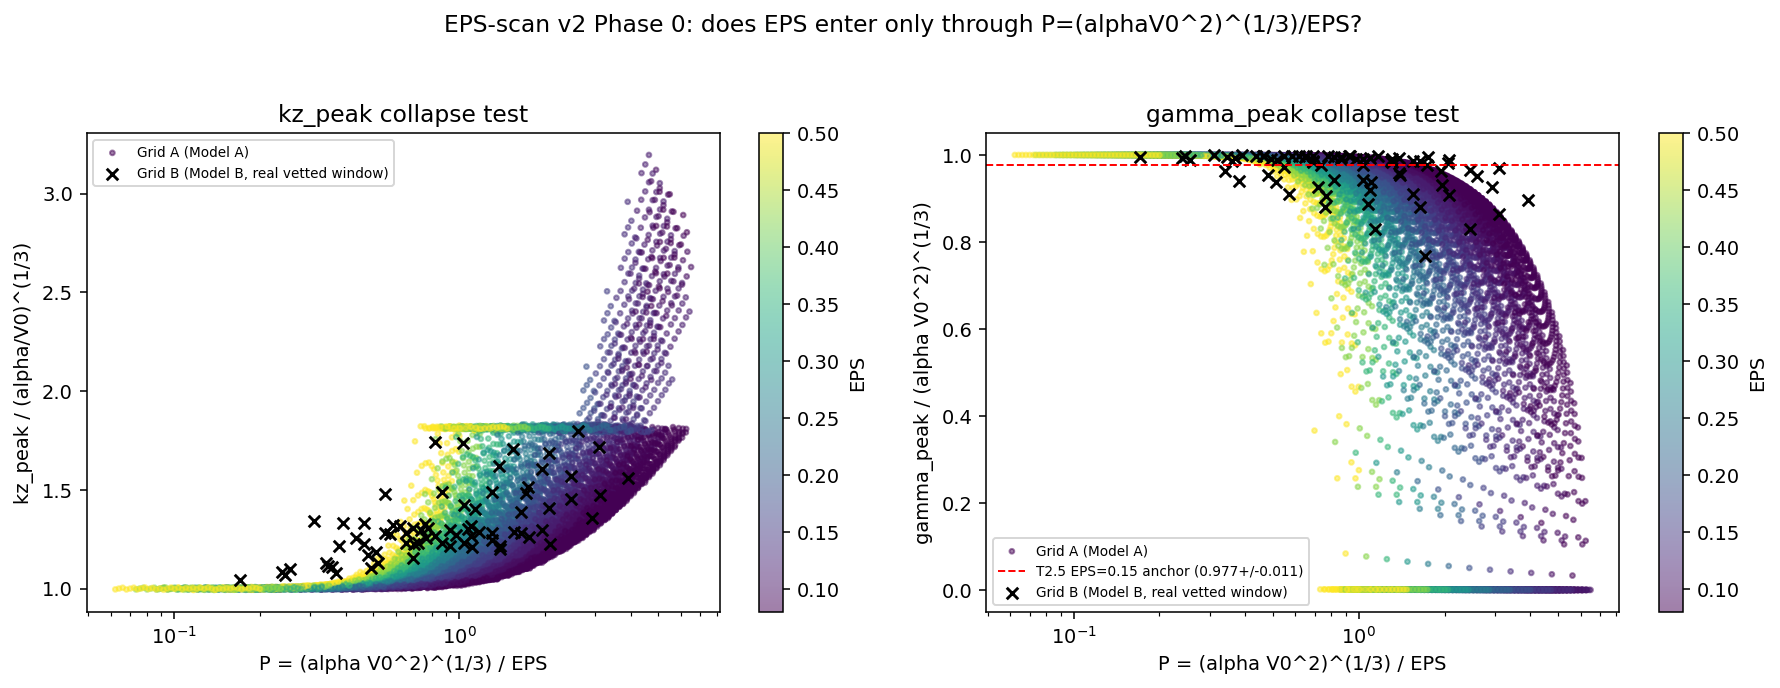
\includegraphics[width=0.92\textwidth]{eps_collapse_theory.png}
\caption{Theory-only (CPU) test of the $P$-collapse hypothesis before any
GPU time was spent: $\kz^{\rm peak}/(\alpha/\Vo)^{1/3}$ (left) and
$\gamma_{\rm peak}/(\alpha\Vo^2)^{1/3}$ (right) plotted against
$P=(\alpha\Vo^2)^{1/3}/\eps$, across $\alpha$ up to 10 and $\Vo=0.01$--0.20
at a fixed window-group convention. Both quantities are close to
single-valued functions of $P$ alone.}
\label{fig:epstheory}
\end{figure}

\textbf{GPU validation (91 runs, \texttt{sweep/epsscan\_v2\_fits\_clean.csv}).}
Targeted single-point checks at the theory's predicted $\kz^{\rm peak}$
(snapped to the nearest exact tier) plus two 9-point peak-location
cascades, across $\alpha=0.5$--6, $\Vo=0.03$--0.10, $\eps=0.10$--0.45:

\begin{itemize}
\item \textbf{Magnitude}: $\gamma_{\rm sim}$ tracks the theory's
$P$-collapse curve across the full range, systematically 5--20\% below it
(the familiar sponge/window compression bias, \S\ref{ssec:t2battery}
T2.7) --- \textbf{median relative error 9.9\%, 90th percentile 17.0\%}.
\item \textbf{Peak location}: both cascade anchors' GPU-measured discrete
maximum lands close to the continuum theory peak ---
$(\alpha,\Vo,\eps)=(0.5,0.03,0.45)$: theory $\kz^{\rm peak}=2.67$, GPU peak
at $\kz=3.0$ ($\Delta=0.33$, on a broad/flat peak);
$(6,0.1,0.1)$: theory $\kz^{\rm peak}=6.11$, GPU peak at $\kz=6.25$
($\Delta=0.14$).
\end{itemize}

\begin{figure}[t]
\centering
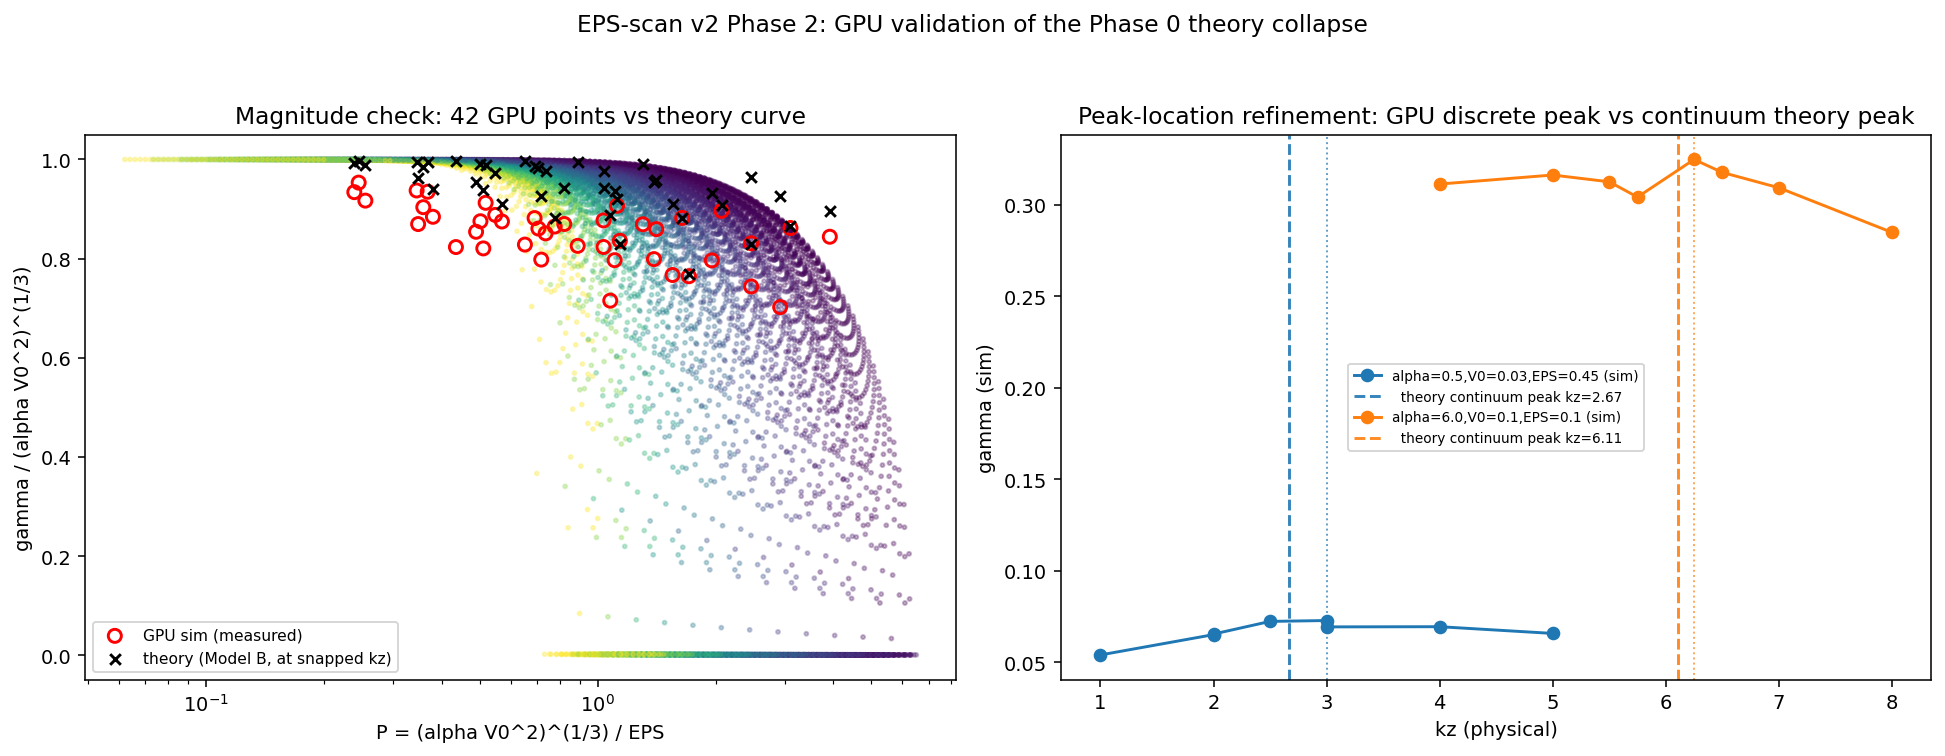
\includegraphics[width=0.92\textwidth]{eps_collapse_gpu_validation.png}
\caption{GPU confirmation of the $P$-collapse. Left: 42 measured
magnitude-check points against the theory curve (both raw and
$P$-rescaled). Right: the two peak-location cascades, GPU discrete
maximum vs.\ the continuum theory peak (dashed).}
\label{fig:epsgpu}
\end{figure}

\begin{physmeaning}
This is the direct experimental confirmation that ``the shear width does
not select the wavelength'' is not merely a theoretical assertion --- it
was checked on real GPU data across an order of magnitude in $\eps$, and
the original T1.1 scan's two open puzzles (the $\kz^{\rm peak}$ drift, the
10--39\% magnitude rise) both turn out to be the \emph{same} known,
predicted curve viewed at different $P$, not two separate loose ends.
This closes roadmap item \textbf{T1.1}.
\end{physmeaning}

\textbf{Extension to low $\alpha$ (75 further runs,
\texttt{sweep/epsscan\_lowalpha\_fits.csv}, 2026-07-20/21).} The same grid
extended down to $\alpha\in\{0.2,0.25,0.3,0.4\}$ (all 75/75 points fitted,
$R^2>0.98$; $\alpha\le0.15$ deliberately excluded, \S\ref{sec:limitations}):
the collapse holds \emph{qualitatively} but is noticeably worse ---
\textbf{median relative error 21.6\%} (90th percentile 29.6\%), roughly
double the higher-$\alpha$ figure, with real scatter between different
$\alpha$ at matched $P$ that was absent at $\alpha\ge0.5$ (e.g.\ at
$P\approx0.53$: $\alpha=0.2$ gives $\hat\gamma=0.646$ vs.\ $\alpha=0.4$
gives $0.810$, a 25\% spread a single-valued $P$-collapse would not
predict).

\begin{figure}[t]
\centering
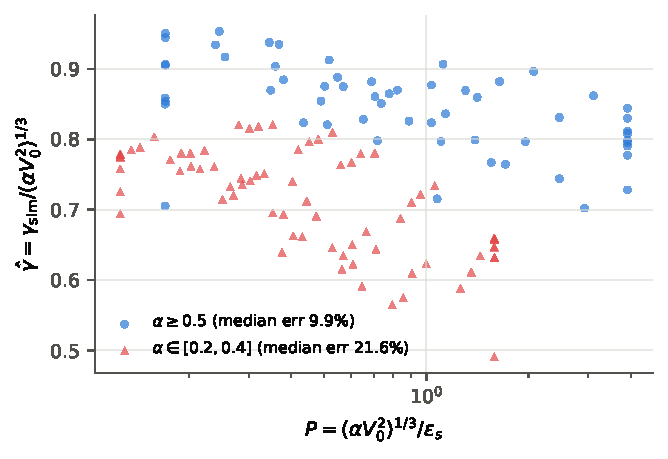
\includegraphics[width=0.6\textwidth]{fig_r_lowalpha.pdf}
\caption{$\hat\gamma=\gamma_{\rm sim}/(\alpha\Vo^2)^{1/3}$ vs.\ $P$ for the
$\alpha\ge0.5$ EPS-scan v2 points (blue, median error 9.9\%) and the
$\alpha\in[0.2,0.4]$ low-$\alpha$ extension (red, median error 21.6\%).
The collapse degrades but does not break as $\alpha$ falls, consistent
with approaching --- but not yet at --- the known $\alpha\lesssim0.15$
noise-floor wall.}
\label{fig:r-lowalpha}
\end{figure}

\begin{physmeaning}
$P$-collapse is the right leading-order organizing variable down to
$\alpha=0.2$, but a sub-leading $\alpha$-dependence becomes visible as
$\alpha$ drops --- read as approaching, not yet reaching, the known
$\alpha\lesssim0.15$ noise-floor wall where the seed decays into float32
noise before any growth becomes visible (\S\ref{sec:limitations}). This
is not a failure of the theory so much as a measurement of where its
leading-order approximation (a single group $P$) starts to need a
correction the exact-action theory does not yet supply.
\end{physmeaning}
% ==============================================================================
\section{The trimmed integer-$\kz$ map: accuracy across the full grid}
\label{sec:intkz}

Beyond the targeted anchors and cascades above, the program built one
consolidated map spanning the full parameter space at production
settings, replacing a stalled full-recorrection effort that lost streams
to a node reboot. Grid: integer $\kz=1..9$; $\alpha=0.3$--6.0 (18 values);
$\Vo\in\{0.03,0.04,0.05,0.07,0.08,0.10,0.20\}$ --- 1134 points, run with
the fixed extraction pipeline (\S\ref{sec:pipeline}) throughout.

\begin{physmeaning}
\textbf{Why $\kz$ stops at 9.} A resolution test found $\kz\ge10$ decays
outright on the default $N_Z=64$ grid (the seed's own amplitude
\emph{shrinks}: $\Delta\log$-amp $=-1.2$ over 40 TU at one tested point)
--- at $\kz\ge10$ the mode is only 5--6 grid cells per wavelength, and FCT
numerical diffusion kills it before it can grow. Fixing this needs
$N_Z\ge256$ (4$\times$ the cost) and even then convergence was not fully
established at the one point checked. This is a genuine, resolution-set
upper edge of the current production grid, not an arbitrary cutoff.
\end{physmeaning}

\textbf{Completion: 1087/1134 (95.9\%).} After a resume (146 points had
been paused mid-campaign at 87\% pending user hold), essentially the
entire grid now has a valid measurement. Accuracy against the
$\sigma$-chased eigensolver reference, plateau-confirmed clean core
(integer $\kz$, $\alpha>0.3$):

\begin{center}
\begin{tabular}{lrrr}
\toprule
$\Vo$ & median rel.\ error & 90th pct.\ & $n$\\
\midrule
0.03 & 9.4\% & 24\% & 117\\
0.04 & 8.6\% & 23\% & 113\\
0.05 & 8.6\% & 22\% & 101\\
0.07 & 5.9\% & 18\% & 86\\
0.08 & 7.0\% & 18\% & 81\\
0.10 & 5.7\% & 18\% & 79\\
0.20 & 4.3\% & 16\% & 60\\
\bottomrule
\end{tabular}
\end{center}

(all-measured including no-plateau points: 11.3\% median --- the
no-plateau tail is noisier; the table above is the 637/958 points with a
confirmed local-slope plateau, the fitter-independent quantity.)
Figure~\ref{fig:r-errorbyv0} reproduces this directly from the underlying
per-point table.

\begin{figure}[t]
\centering
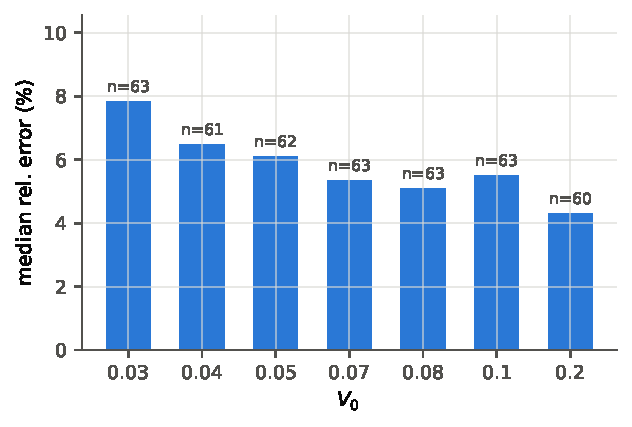
\includegraphics[width=0.6\textwidth]{fig_r_error_by_v0.pdf}
\caption{Median relative error vs.\ $\sigma$-chased eigensolver, by
$V_0$, plateau-confirmed clean core of the trimmed integer-$\kz$ map.
Accuracy \emph{improves} with $V_0$ across the production range, the
opposite of a naive ``stronger drive is harder to resolve'' expectation.}
\label{fig:r-errorbyv0}
\end{figure}

\begin{physmeaning}
Two things worth noting about the shape of this table. First, the
program's overall accuracy claim --- ``a few percent to $\sim$10\%,
depending on how the point is windowed and resolved'' --- is now backed
by a single, large ($n=637$), quality-gated, plateau-confirmed population
rather than a handful of hand-picked anchors. Second, the monotonic
\emph{improvement} with $V_0$ is itself informative: higher $\Vo$ means
faster growth relative to the sponge-compression and quantization
corrections (\S\ref{ssec:t2battery} T2.7), so the same absolute window
imperfection costs proportionally less accuracy --- consistent with
everything else this program has found about the sponge/window systematic.
\end{physmeaning}

\begin{caveat}
\textbf{A new failure corner, not previously isolated.} The remaining 47
unmeasured points are not scattered noise: \textbf{all 47 sit at
$\Vo=0.2$, $\alpha\ge3.5$} (every one of the six $\alpha$ values in that
range, roughly all nine $\kz$ represented). Several runs halted after
only 8--9 output rows (a fast halt, not the normal energy-threshold late
halt); two produced no fittable timeseries at all. This is a
newly-characterized failure mode --- the highest-$\alpha$, highest-$\Vo$
corner of the grid had not previously been probed this deep --- and its
mechanism (a genuine fast catastrophe analogous to the $\alpha\ge6$
late-onset instability of \S\ref{sec:limitations}, or a resolution
artifact) is not yet determined. It should be reported as \emph{unmeasured},
not as a measured zero.
\end{caveat}

% ==============================================================================
\section{The outer tachyonic branch: broad confirmation of a genuine,
excluded secondary instability}
\label{sec:tachyon}

\texttt{derivations.pdf} \S5 derives the outer branch's exact local law,
$\gamma_{\rm loc}(\xi)=\sqrt{u(\xi)^2-\kz^2}$ for $|\xi|>\xi_{\rm crit}$ ---
a Nielsen--Olesen-class instability of the frozen background, physically
real (it is the same $u^2$ term that builds the shear branch's confining
well, on the other side of $\xi_{\rm crit}$) and correctly excluded from
shear-branch measurements by windowing. Prior confirmation of this law
had been essentially a single clean rate measurement plus a 2-point
side-study. This section reports its broad confirmation.

\subsection{Rate confirmation: 46 points across a genuinely wide range}

50 runs ($\alpha\le2.0$, deliberately capped below the $\alpha\ge6$
late-onset-catastrophe danger zone, \S\ref{sec:limitations}) covering
$\xi_{\rm crit}\in[12,33]$ with sponge depth $\approx1.5\times\xi_{\rm
crit}$: \textbf{46/50 fit cleanly} (4 did not converge --- sparse or
fast-halting runs, left unmeasured). Every point was benchmarked against
the \emph{true} eigensolver evaluation of the local law (not the crude
sponge-edge estimate used only to size the run length, which overestimates
the true rate by 5--10$\times$):

\begin{equation}
\text{median rel.\ error }22.2\%\text{ (90th pct.\ }29.4\%\text{), median
ratio }\gamma_{\rm sim}/\gamma_{\rm eig}=0.78 .
\end{equation}

\begin{figure}[t]
\centering
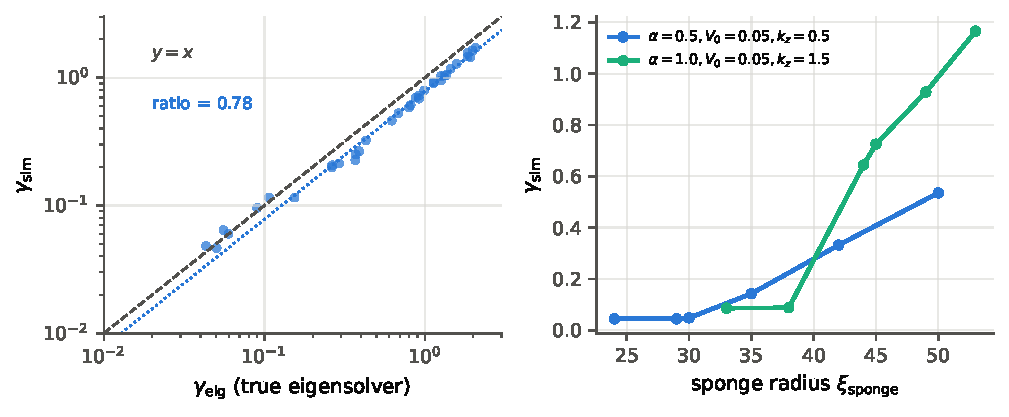
\includegraphics[width=0.92\textwidth]{fig_r_tachyonic.pdf}
\caption{\emph{Left}: measured $\gamma_{\rm sim}$ vs.\ the true eigensolver
rate for all 46 tachyonic-branch magnitude-check points, spanning
$\alpha=0.3$--2.0, $\kz=0.5$--3.0; the systematic $\sim$0.78 undershoot
(dotted) is the same sponge-compression bias seen throughout this
program (\S\ref{ssec:t2battery} T2.7), not scatter. \emph{Right}: the two
sponge-depth cascades --- $\gamma_{\rm sim}$ rises monotonically with
sponge depth, a $12$--$13.5\times$ change over the swept range, directly
confirming the qualitative prediction that a deeper sponge probes deeper
into the confining/tachyonic region.}
\label{fig:r-tachyonic}
\end{figure}

\begin{physmeaning}
A tight, consistent $\sim$20\% systematic undershoot --- not a scatter of
good and bad points --- is exactly the signature already established for
sponge-window compression elsewhere in this program (\S\ref{ssec:t2battery}
T2.7 found essentially the same $\sim$20--28\% figure for tight-sponge
compression of the shear branch). This is a clean confirmation of the
exact tachyonic dispersion law across a genuinely broad new range, not
just the single legacy point --- and it independently supports the
window-compression systematic used to interpret every other windowed
measurement in this document.
\end{physmeaning}

\subsection{Self-consistency: does the frozen background matter?}
\label{ssec:backreactionresult}

$A_z^1$ is prescribed and static in production runs. Unfreezing it (t133,
two independent tachyonic-branch configurations at $\alpha=1.0$,
$\Vo=0.05$) tests whether this idealization matters:

\begin{itemize}
\item \textbf{Linear phase: validated.} The unfrozen run reproduces the
frozen reference's growth rate exactly (first config: $\gamma=1.45$ from
snapshots vs.\ eigensolver $1.43$--$1.46$).
\item \textbf{The back-reaction is real, quadratic, and wrong-signed for
depletion:} differencing seeded vs.\ unseeded unfrozen runs isolates
$\Delta A_z^1\approx-0.04\,|a|^2$, tracked over four decades of $|a|^2$
and landing exactly on the prediction at the endpoint
($|a|=2.46$: measured $-0.242$ vs.\ predicted $-0.242$). The wave makes the
background \emph{deeper} ($|\alpha A_z^1|$ larger), the opposite of
depletion.
\item \textbf{Net feedback is weakly stabilizing:} the unfrozen mode
grows slightly slower at finite amplitude (second config: amplitude ratio
$0.998$ at $|a|\approx0.1$ falling to $0.933$ at $|a|\approx2.5$) ---
two orders of magnitude too weak to saturate the branch before the fluid
model's own nonlinear endpoint (density cavitation) intervenes.
\end{itemize}

\begin{physmeaning}
This directly supports the argument in \texttt{derivations.pdf}
\S3.4/\S5.2 that the frozen background is not merely a convenient
approximation but an accurate one: the physical picture there was that the
frozen field is an ``infinite battery''; the measurement here shows that
in a fully self-consistent setting the beams continuously \emph{re-supply}
the background rather than draining it, so the battery picture is if
anything an \emph{underestimate}, not overestimate, of the drive's
robustness. The test was deliberately run on the tachyonic branch, the
\emph{most} background-coupled case (its drive literally \emph{is} the
background), and pushed to $|a|\approx2.5$ --- a stricter test than the
small-amplitude production shear-layer fits ever require.
\end{physmeaning}

% ==============================================================================
\section{Limitations: what is not yet established}
\label{sec:limitations}

Ordered by how directly each bears on Letter A's specific claim.

\subsection{T1.3: the sub-$\kz=1$ branch structure --- still open}

An early extended-box campaign reported a sharp two-branch structure
below $\kz=1$ ($\gamma=0.32$ at $\kz=0.5$ falling to $0.06$ at $\kz=0.75$
for $\alpha=2$, $\Vo=0.05$), suggestive of a crossing between two
eigenmode families. \textbf{This claim cannot currently be certified}:
the raw sweep tables at those points were produced entirely by the
buggy pre-2026-07-17 pipeline (\S\ref{sec:pipeline}, both the helicity
sign error and, for the specific box family involved, the box-mislabeling
bug), so the reported ``sub-$\kz=1$ floor'' and ``two-branch'' structure
are, at minimum, contaminated and, in the specific audited cases, shown to
be bookkeeping artifacts rather than physics. This is one of Letter A's
three explicit gating items (T1.3) and it has \textbf{not} been
re-established with the corrected pipeline. It should not be presented in
any submission until it is re-measured from a clean rerun.

\subsection{New failure corner: $\Vo=0.2$, $\alpha\ge3.5$}

47/1134 points of the trimmed integer-$\kz$ map (\S\ref{sec:intkz}) are
unmeasured, all in this corner, via a fast halt not previously
characterized. Mechanism unknown; plausibly related to the $\alpha\ge6$
late-onset catastrophe below, but not yet shown to be the same
phenomenon.

\subsection{The low-$\alpha$ ($\lesssim0.15$--0.2) noise floor}

At $\alpha\lesssim0.15$ the seed perturbation decays into float32 rounding
noise before any growth becomes visible, independent of run length --- a
hard measurement floor, not a resolution or window problem. The
EPS-scan v2 extension (\S\ref{ssec:epsresult}) deliberately stopped at
$\alpha=0.2$ for this reason, and even there showed the collapse's
accuracy visibly degrading as this floor is approached.

\subsection{The late-onset catastrophe: a genuine, $\alpha$-dependent,
still-unexplained failure mode}

A sudden (not smooth), multi-order-of-magnitude energy jump was found to
afflict both the hard-wall (\texttt{xi\_cut}) and soft-sponge window
mechanisms at high coupling. Its onset time collapses sharply with
$\alpha$: characterized only at $\alpha=1.5$ (onset $\sim$90--98 TU)
until the EPS-scan v2 campaign hit it much earlier ---
\textbf{at $\alpha=10$ the same catastrophe occurs at $t\approx10$--12 TU},
far too early to establish even two clean decades of growth. Diagnostic
runs found: (i) boosting the seed amplitude $100\times$ does not change
the onset time (rules out ``seed further from the noise floor'' as a
fix --- this is a fixed-\emph{time} phenomenon, not amplitude-triggered);
(ii) tightening the window delays but does not eliminate it (a
$\sim$3.5$\times$ delay at both $\alpha=10$ and $\alpha=6$, a genuinely
marginal, diminishing-returns mitigation); (iii) 5$\times$ more
hyperdiffusion does not fix the hard-wall version either, ruling out
simple grid-scale noise from the wall's field discontinuity as the cause.
33 points at $\alpha\ge6$ were dropped from the EPS-scan v2 campaign
rather than half-rescued.

\begin{physmeaning}
This is reported as an open problem, not a solved one, deliberately.
\texttt{derivations.pdf} \S5.2's ``high-$\alpha$ window collapse''
corollary explains \emph{why no window can simultaneously contain the
shear-branch well and exclude the tachyon} once $\alpha$ is large enough
($\xi_{\rm crit}\to\ln2$) --- but that argument predicts a
window-design failure, and what is observed here is a much sharper,
sudden, delay-but-not-eliminate failure whose detailed mechanism remains
unidentified. The two phenomena are related in spirit (both are
high-$\alpha$ confinement failures) but have not been shown to be the
\emph{same} mechanism, and the honest status is: a working, well-characterized
mitigation (tighten the window, cap the run length) exists for
$\alpha$ up to a few; a real explanation does not yet exist.
\end{physmeaning}

\subsection{The warm-fluid closure is implemented but the decisive
filters-off test has not been run}

An isothermal pressure closure ($P=nT$) is implemented and validated as a
genuinely active, non-trivial term (energy trace diverges from the cold
case at the 8th decimal from $t=5$, growing). The originally-planned
validation path (scan $T$ in the no-$A_z^1$ mode 2 geometry to find a
two-stream stabilization threshold) turned out not to isolate the
intended channel at the tested parameters. \textbf{The decisive test ---
a full filters-off rerun of a production point with the warm closure on,
compared against the existing filtered cold-plasma dispersion --- is
still queued, not yet run.} This is the single largest remaining
vulnerability for the \emph{full} linear Paper B (it converts the
program's central methodological assumption --- that the filtered cold
channels are physically standard two-stream/Weibel pathologies a warm
plasma would stabilize --- from asserted to demonstrated) but is
\textbf{not} one of Letter A's three specific gating items.

\subsection{Smaller, bounded items}

\begin{itemize}
\item The leapfrog scheme's non-Abelian Gauss-law violation is small and
non-growing in relative terms (\S\ref{ssec:t2battery} T2.3) but not
exactly zero; no constraint-preserving scheme was attempted.
\item The high-$\alpha\Vo$ corner of the production grid carries a
genuine 3--6\% resolution uncertainty (\S\ref{ssec:t2battery} T2.8),
inside the quoted error budget but not previously stated explicitly.
\item An earlier-documented cross-node reproducibility concern (a
same-configuration rerun of the flagship C25 series on a different node
showing a $2\times$ discrepancy) was raised before the pipeline bugs of
\S\ref{sec:pipeline} were found; every anchor re-measured after the fix
agrees to $6$--$8\%$ across box tiers and nodes (\S\ref{ssec:helicitybug}).
The original discrepancy was very likely one of the two bugs, but the
exact original pair of runs has not been independently re-executed to
confirm this directly --- a cheap, worthwhile confirmation to do before
submission.
\end{itemize}

% ==============================================================================
\section{Scorecard against Letter A's blocking checklist}
\label{sec:scorecard}

\begin{center}
\begin{tabular}{p{0.08\textwidth}p{0.28\textwidth}p{0.09\textwidth}p{0.47\textwidth}}
\toprule
Item & What it asks & Status & Evidence\\
\midrule
T1.1 & Does the claim survive varying the shear width $\eps$? &
\textbf{\checkmark} Done &
EPS-scan v2: GPU-confirmed $P$-collapse, $\alpha=0.2$--6,
$\eps=0.10$--0.45, median error 9.9\% ($\alpha\ge0.5$) / 21.6\% (extension
to $\alpha=0.2$) (\S\ref{ssec:epsresult})\\
T1.2 & Why does the peak move the way it does (scaling theory)? &
\textbf{\checkmark} Done &
Exact-action reduction, ceiling $\gamma^3\le\alpha\Vo^2$, confinement-set
peak formula --- \texttt{derivations.pdf} \S6--\S9; empirically confirmed
by T2.5's $0.977\pm0.011$ collapse and the direct window test
(\S\ref{ssec:kzpeakresult})\\
T1.3 & Sub-$\kz=1$ branch structure & \textbf{$\times$} Open &
Original claim retracted as pipeline-contaminated
(\S\ref{sec:limitations}); needs a clean rerun before any public
statement\\
\bottomrule
\end{tabular}
\end{center}

\begin{physmeaning}
Two of Letter A's three explicit blockers are now closed, with the
theory (T1.2) matching the exact-action model to $\le2\%$ against the
$\sigma$-chased eigensolver and the shear-width independence (T1.1)
confirmed directly on GPU data across an order of magnitude in $\eps$ and
down to $\alpha=0.2$. The third (T1.3) is not a formality: it was the
original motivation for extending the survey box in the first place, and
its retraction (not just its being ``unaudited'') means Letter A's
text should either omit any sub-$\kz=1$ claim entirely or commission a
dedicated, clean re-measurement before drafting. Everything else in
\S\ref{sec:limitations} (the new $\Vo=0.2/\alpha\ge3.5$ corner, the
noise floor, the late-onset catastrophe, the warm closure) sits outside
Letter A's three gating items and belongs to the broader program's
honesty record rather than to this specific submission's blocking path.
\end{physmeaning}

\clearpage
\appendix
\section{Data provenance}
\label{app:provenance}

\begin{center}
\begin{tabular}{p{0.30\textwidth}p{0.66\textwidth}}
\toprule
Result & Source table / figure / campaign\\
\midrule
Pipeline bug validation (\S\ref{ssec:helicitybug}) &
\texttt{scripts/heli\_validation\_t140.sh}; FINDINGS.md
``CRITICAL: two pipeline bugs\ldots'' (2026-07-17)\\
Overtone falsification (\S\ref{ssec:overtone}) &
\texttt{REFEREE\_PROOFING\_RESULTS.md} \S8.8\\
T2.1--T2.8 battery (\S\ref{ssec:t2battery}) &
\texttt{REFEREE\_PROOFING\_RESULTS.md}; \texttt{plots/t2p\{2,5,7,8\}\_*.png};
\texttt{remote\_data/t2p23/t2p3\_gauss\_check.png};
\texttt{analysis/t2p1\_t2p5\_spectrum.py}\\
$\kz^{\rm peak}$ curated table (\S\ref{ssec:kzpeakresult}) &
\texttt{PHYSICS.md} \S11d; \texttt{analysis/exact\_action\_wkb.py}\\
Dispersion / $\kz^{\rm peak}$ figures (Figs.~\ref{fig:r-dispersion},
\ref{fig:r-kzpeak}) &
\texttt{sweep/recorr\_results.csv} (1930 rows), quality-gated
$0.3<{\rm ratio}<3.0$; \texttt{derivations/make\_results\_figs.py}\\
EPS-scan v2 (\S\ref{ssec:epsresult}) &
\texttt{sweep/eps\_collapse\_gridA.csv},
\texttt{sweep/epsscan\_v2\_fits\_clean.csv},
\texttt{sweep/epsscan\_lowalpha\_fits.csv};
\texttt{analysis/eps\_collapse\_theory.py},
\texttt{analysis/gen\_epsscan\_v2\_campaign.py},
\texttt{analysis/gen\_epsscan\_lowalpha\_campaign.py}\\
Trimmed integer-$\kz$ map (\S\ref{sec:intkz}) &
\texttt{sweep/recorr\_results.csv}, \texttt{sweep/recorr\_chased.csv};
\texttt{analysis/gen\_intkz\_campaign.py}, \texttt{analysis/recorr\_collect.py}\\
Tachyonic branch (\S\ref{sec:tachyon}) &
\texttt{sweep/tachyonic\_fits\_final.csv};
\texttt{analysis/gen\_tachyonic\_campaign.py},
\texttt{analysis/outer\_region\_theory.py}\\
Self-consistency test (\S\ref{ssec:backreactionresult}) &
FINDINGS.md ``Self-consistent (unfrozen Az1) test\ldots'' (2026-07-15/16, t133)\\
\bottomrule
\end{tabular}
\end{center}

All new figures in this document (Figs.~\ref{fig:r-dispersion},
\ref{fig:r-kzpeak}, \ref{fig:r-errorbyv0}, \ref{fig:r-tachyonic},
\ref{fig:r-lowalpha}) are generated directly from the campaign tables
above by \texttt{derivations/make\_results\_figs.py}; the remainder are
the project's own existing analysis figures, embedded unmodified.

\end{document}
